%objetivos.tex

\section{Objetivos}
\label{sec:objetivos}

Según lo expuesto en la sección \ref{sec:intro}, sería deseable disponer de
un sistema que simule una constelación de satélites y varias estaciones de tierra con sus respectivas métricas en las comunicaciones. Además, que el procesado de los datos en bruto obtenidos en las estaciones de tierra se realice en la nube y la adquisición de esas imágenes procesadas por parte de los clientes sea real.

\begin{figure}
\begin{center}
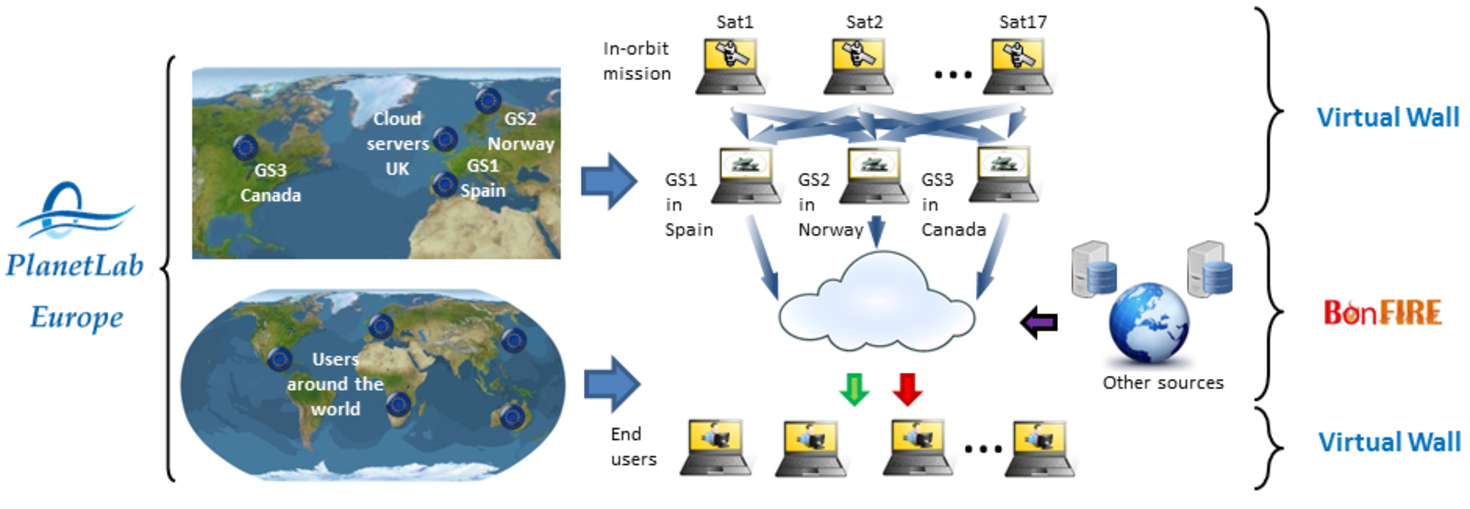
\includegraphics[width=.9\textwidth]{GEOCloud_in_Fed4FIRE.pdf}
\caption{Geo-Cloud en Fed4FIRE. Imágen obtenida de Fed4FIRE Federation}
\end{center}
\end{figure}

Por ello en este proyecto se plantean los siguientes objetivos:

\begin{itemize}

\item \textbf{Implementación de los servicios basados en Cloud en la plataforma BonFIRE:}  Se pretende desarrollar un servicio de procesamiento de datos Raw y creación de imágenes ortorectificadas en Cloud. Para esta implementación será necesario conocer la arquitectura de la cadena de procesado que se implementa en Elecnor Deimos. Además se debe dar soporte a las peticiones de los clientes con lo cuál se deben de implementar servicios de distribución de estos resultados entre los usuarios finales.

\item \textbf{Implementación de la constelación de satélites, estaciones de tierra y clientes sobre PlanetLab Europe:}  Para esto se usará PlanetLab Europe, con la que conseguiremos simular conexiones de red entre distintos nodos distribuidos por el mundo.
A tavés de la implementación del modelo de red en PlanetLab Europe se podrán medir las características de una red real. Se realizarán dos capas en esta implementación. La primera modelará las estaciones de tierra y la constelación; la segunda, los clientes finales accediendo a los servicios Cloud.

\item \textbf{Implementación de la constelación de satélites, estaciones de tierra y clientes sobre VirtualWall:} Tras realizar la implementación sobre PlanetLab Europe, se conseguirá toda la información de una red real, con lo que se realizará un modelo sobre VirtualWall de acuerdo a esos parámetros. Además esta plataforma permitirá tener completo control sobre los recursos y todos los factores envueltos en los distintos casos de prueba, con lo que se podrá evaluar su comportamiento.

\item \textbf{Simulación de distintos escenarios y obtención de resultados:} Tras realizar la implementación de lo anteriormente expuesto, se procederá a realizar uno o varios casos de prueba con los que obtengamos datos para contrastar cómo actúa este servicio de procesado de obtención de geo-imágenes en la nube.



\end{itemize}







% Local Variables:
%   coding: utf-8
%   fill-column: 90
%   mode: flyspell
%   ispell-local-dictionary: "castellano"
%   mode: latex
%   TeX-master: "main"
% End:
